\chapter{Goal Oriented Action Planning}

Das Goal Oriented Action Planning Planung Entscheidungssystem ist zur Planung zu einem bestimmten Ziel gedacht. Planung ist der Prozess der Suche einer Sequenz an Aktionen zur Erreichung eines Zieles. Die Suche kann dabei als Suchproblem dargestellt werden. Für das Verständnis wird daher Kenntnis der Themen Suchalgorithmen und Suchprobleme benötigt.



\section{Historie}

Das Entscheidungssystem \textit{Goal Oriented Action Planning} (\textit{GOAP}) entstand in der Entwicklung des Videospiel \textit{F.E.A.R First Encounter Assault Recon (2005)}. Die Entwickler wollten ein Videospiel entwickeln, das wie ein Actionfilm wirkt, mit intensiven Kämpfen. Für die intensiven Kämpfe benötigt man NPC, welche Deckung nehmen, blind feuern, über Fenster springen, Granaten werfen, untereinander kommunizieren und weitere Aktionen ausführen können.

Zuvor nutzte \textit{Monolith} Finite State Machines (\textit{FSM}) als Entscheidungssystem. Den Entwicklern fiel es jedoch zunehmend aufwendig, eine FSM mit neuen Zuständen und den dazugehörigen Aktionen zu erweitern. In einem vorherigen Videospiel \textit{No One Lives Forever (2000)}, wurde veruscht eine dynamische FSM zu implementieren, die sich an Zielzustände anpassen konnte. Allerdings wurde auch diese Lösung als zu unflexibel wahrgenommen. Aus dem Versuch der dynamischen FSM und STRIPS hat Jeff Orkin das GOAP System entwickelt, welches Echtzeitplanung erfüllen soll. Eine der Herausforderungen, mit denen sich Jeff Orkin während der Entwicklung konfrontiert sah, war die Berücksichtigung der Performance.\autocite{retro_fear}



\section{GOAP Bestandteile}

Das GOAP -System basiert dabei auf dem STRIPS System. Wie auch STRIPS besitzt GOAP Ziele, welche einen gewünschten Zustand beschreiben und Aktionen mit Effekten die Zustände ändern können. GOAP sucht nach einer Sequenz an Aktionen die das Ziel des NPC erreichen kann. Im Sinne von Jeff Orkins geschieht die eigentliche Ausführung der Aktionen über eine Finite State Machine (\textit{FSM}).


\subsection{Finite State Machine in GOAP}

Eine FSM wurde im Videospiel \textit{F.E.A.R} für die Ausführung der Aktionen benötigt. Die NPC führten ihre Aktionen durch eine Kombination aus Animationen und Bewegungen aus. Beispielsweise sorgte eine Cover-Aktion dafür, dass der NPC hinter eine Deckung lief und dort eine Deckungs-Animation abspielte. Eine Shoot-Aktion hingegen aktivierte eine entsprechende Schuss-Animation. Die FSM bestand dabei aus den drei Zuständen GoTo, Animate und UseSmartObject. 
\begin{figure}[h]
  \centering
  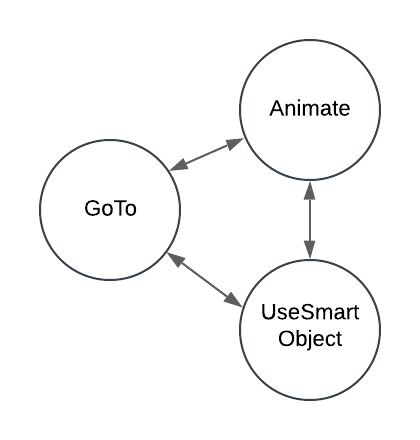
\includegraphics[width=7cm]{GOAP/GOAP_FSM}
	\captionsetup{justification=justified, format=plain}
  \caption{GOAP Finite State Machine}
  \label{GOAP_FSM}
\end{figure}

\textit{Monolith} hat durch die Zustände \textit{Animate} und \textit{UseSmartObject} Animationen umgesetzt. Der Unterschied zwischen den beiden Zuständen bestand darin, dass \textit{UseSmartObject} Animationen steuerte, die von \textit{SmartObjects} in der Spielwelt vorgegeben wurden, während \textit{Animate} Animationen abspielte, die direkt im NPC gespeichert waren. Der Zustand \textit{GoTo} hat ebenfalls Animationen abgespielt, kombinierte diese jedoch mit der tatsächlichen Bewegung des NPCs durch die Spielwelt.

Die Zustandswechsel wurden durch die Aktionen bestimmt, welche wiederum durch GOAP gegeben wurden.


\subsection{GOAP Ziele}

Ein Ziel $GOAL(g)$ in GOAP setzt die erwünschte Zielzustände für den Planer. So setzt das Ziel $EliminatePlayer$ den Zielzustand $\{\lnot PlayerAlive\}$.
\[
	\highlightbox{0.9\textwidth}{$
		\begin{align*}
			GOAL(EliminatePlayer) = \{\lnot PlayerAlive\}
		\end{align*}
	$}
\]

Die Auswahl des Zieles geschieht nach ihrer Priorität und ob dieses gültig ist. Das Ziel mit der höchsten Priorität und Gültigkeit wird bevorzugt. Die Gültigkeit und Priorität basiert dabei auf dem Zustand $s$ des NPC und seiner Umwelt.
\[
	\highlightbox{0.9\textwidth}{$
		\begin{align*}
			s = \{\lnot PlayerVisible\} \\
			PRIORITY(s,EliminatePlayer) = 100 \\
			VALID(s,EliminatePlayer) = false
		\end{align*}
	$}
\]


\subsection{GOAP Aktionen}

Aktionen können Weltzustände oder auch direkte Zustände eines NPC ändern. So kann beispielsweise die Aktion \textit{Reload} den Zustand $s = \{\lnot GunLoaded\}$ ändern.
\[
	\highlightbox{0.9\textwidth}{$
		\begin{align*}
			TRANSITIONS(s,Reload) &= \{GunLoaded\}
		\end{align*}
	$}
\]

Dadurch haben Aktionen die Möglichkeit Zielzustände zu erreichen. Nehmen wir an der NPC hat das Ziel $Patrol$ und die Aktion $GoPatrol$ mit $TRANSITIONS(s,GoPatrol) = {AtPatrol}$, dann kann diese Aktion den Zielzustand erreichen.

Eine Aktion hat auch Vorbedingungen als Zustände, diese Zustände können wiederum von anderen Aktionen erfüllt werden. So könnte beispielsweise die Aktion $Reload$ die Vorbedingung der Aktion $Shoot$ erreichen.
\[
	\highlightbox{0.9\textwidth}{$
		\begin{align*}
			PRECONDITION(Shoot) = \{GunLoaded\}
		\end{align*}
	$}
\]

Eine Aktion setzt auch wie im Suchproblem eine $ACTIONCOST$ Funktion um, die später zur Auswahl einer Aktion herangezogen wird. Wird die Aktion ausgewählt wird diese später von der FSM ausgeführt.


\subsubsection{Fallbeispiel}

Nehmen wir an, dass der NPC den Ausgangszustand $s_a$ und das Ziel $EliminatePlayer$ besitzt.
\[
	\highlightbox{0.9\textwidth}{$
		\begin{align*}
			s_a = \{PlayerVisible, \lnot GunLoaded\, \lnot AtCover\} \\
			GOAL(EliminatePlayer) = \{\lnot PlayerAlive\}
		\end{align*}
	$}
\]

Der NPC muss nun versuchen das Ziel mit den möglichen Aktionen den Zielzustand $\{\lnot PlayerAlive\}$ erreichen. Die möglichen Aktionen werden dabei aus einer $ACTIONS(s)$ Funktion gelesen.
\[
	\highlightbox{0.9\textwidth}{$
		\begin{align*}
			ACTIONS(s) = \{Reload, MoveToCover\} \\
			TRANSITIONS(s,Reload) = \{GunLoaded\} \\
			TRANSITIONS(s,MoveToCover) = \{AtCover\}
		\end{align*}
	$}
\]

Aus der $TRANSITIONS$ Funktion können wir entnehmen, dass keine der Aktionen den Zustand $\lnot PlayerAlive$ direkt erreichen kann. Es muss ein Zustand entdeckt werden aus dem mit einer entsprechenden Aktion das Ziel erreicht werden kann. Eine Lösung wäre \textit{Brute Force}, das durchgehen aller möglichen Aktionen bis letztlich das Ziel gefunden wird. Dies sorgt jedoch für einen hohen Rechenaufwand bei komplexen NPC mit vielen Aktionen und Zuständen. Außerdem können beim Brute Force suboptimale Sequenzen an Aktionen gefunden werden, da dieser die Kosten der Aktionen nicht beachtet. In GOAP sucht der A* Suchalgorithmus über den GOAP Planner die optimale Sequenz an Aktionen zum erreichen des Zieles.


\subsection{GOAP Planner}

Der GOAP Planner ist dabei die eigentliche Lösung des Suchproblems. Der Planner bestimmt das Ziel mit der höchsten Priorität und Gültigkeit. Die dazugehörige Sequenz wird über den A* Suchalgorithmus im GOAP Planner gesucht. Der A* Suchalgorithmus wird im Kapitel Suchalgorithmen ausführlich beschrieben.

Der A* ist in der Videospiel-Entwicklung für die Suche des Navigation-Pfades bekannt. Er kann aber auch für andere Suchprobleme genutzt werden, wie für die Suche einer Aktion-Sequenz. Wie auch für die Navigation erzeugt A* einen Suchbaum, mit dem Unterschied, dass die Knoten Zustände sind, die durch die Kanten also Aktion-Effekte erzeugt werden.

\begin{table}[h]
  \caption{A* Vergleich für Navigation und Aktion-Plannung}
  \label{A*: Vergleich}
  \renewcommand{\arraystretch}{1.2}
  \centering
  \small
    \begin{tabularx}{0.95\textwidth}{X X X}
      \toprule
      \textbf{A*} & \textbf{Navigation} & \textbf{Aktion-Plannung}\\
      \toprule
      Knoten & NavMesh Polygon & Zustand &
			Kanten & NavMesh Polygon Kanten & Aktionen &
      \bottomrule
    \end{tabularx}
\end{table}


\subsubsection{Bewertungsfunktion in der Aktions-Planung}

Es ist zwar möglich aus dem Ausgangszustand zu suchen, könnte aber einem \textit{Brute Force} ähneln und dadurch ineffizient sein. Die Aktion wird nicht wie bei der Navigation vom Ausgangszustand ausgewählt, sondern aus dem Zielzustand $s_z$ aus. Von dort aus wird die Suche nach Aktionen fortgesetzt, die die Vorbedingungen der zuvor gewählten Aktion erfüllen. Die Suche wird fortgesetzt bis alle Vorbedingungen von Aktionen erfüllt wurden. Der Planer speichert dabei die Auswahl der Aktionen in einer Sequenz ab.

%---------------------------------------------------------------------------------------------------------------------------------------

\section{Beispiel}

Wir setzten das Beispiel mit dem Wissen über den GOAP Planner fort.
\[
	\highlightbox{0.9\textwidth}{$
		\begin{align*}
			s_a = \{PlayerAlive, PlayerVisible, \lnot AtPatrol, \lnot GunLoaded\, \\
			\lnot AtCover, \lnot AtPlayer,  \lnot AtLastPlayerPostion\}
		\end{align*}
	$}
\]


\subsubsection{Auswahl des Zieles}

\begin{table}[h]
  \caption{Ziel Tabelle}
  \label{Kap4:Ziel}
  \renewcommand{\arraystretch}{1.2}
  \centering
  \small
    \begin{tabularx}{0.95\textwidth}{X X X X}
      \toprule
      \textbf{Goal} & \textbf{Ziel-Zustand} & \textbf{Gültigkeit} & \textbf{Priorität}\\
      \toprule
      EliminatePlayer & \lnot$ PlayerAlive & true & 3 \\
			SearchEnemy & AtLastPlayerPostion & true & 1 \\
			Patrol & \lnot$ AtPatrol & false & 2 &
      \bottomrule
    \end{tabularx}
\end{table}

Der GOAP Planer wählt das Ziel mit der höchsten Priorität und Gültigkeit. Nehmen wir an, dass das Ziel \textit{Patrol} aufgrund der \textit{VALID(s,Patrol)} Funktion nicht gültig ist, so würde das Ziel ausfallen. Es verbleiben die Ziele: \textit{EliminatePlayer} und \textit{SearchEnemy}. Da \textit{EliminatePlayer} mit $PRIORTIY(s,EliminatePlayer) = 3$ die höhere Priorität hat, wird diese als Ziel ausgewählt.

\subsubsection{Suche nach der Aktion-Sequenz}

\begin{table}[h]
  \caption{Aktionen ihre Effekte und Vorausgesetzte Zustände}
  \label{Kap4:Aktionen}
  \renewcommand{\arraystretch}{1.2}
  \centering
  \small
    \begin{tabularx}{0.95\textwidth}{l l l l}
      \toprule
      \textbf{Aktion} & \textbf{Effekt} & \textbf{Vorausgesetzte Zustände} & \textbf{Kosten}\\
      \toprule
      Shoot & \lnot$ PlayerAlive & GunLoaded, PlayerVisible & 1\\
			Melee & \lnot$ PlayerAlive & AtPlayer, PlayerVisible & 3\\
      Reload & GunLoaded & \lnot$ GunLoaded & 1\\
      GoTo & AtCover, AtPlayer & - & 10 \\
			Heal & Healed &  AtCover & 1 &
      \bottomrule
    \end{tabularx}
\end{table}
$

Der Algorithmus erstellt nun einen Suchbaum. Der Wurzelknoten im Suchbaum speichert, dabei den erwünschten Zielzustand des Zieles. Im Falle des Beispiels ist der Zielzustand $s_z = GOAL(EliminatePlayer) = \{\lnot PlayerAlive\}$.

\begin{figure}[h]
  \centering
  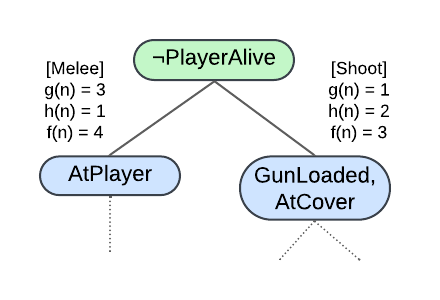
\includegraphics[width=10cm]{GOAP/GOAP_1}
	\captionsetup{justification=justified, format=plain}
  \caption{GOAP A* Suche: Grüne Knoten sind Knoten, welche erweitert wurden. Blaue Knoten sind Knoten aus der offenen Liste.}
  \label{GOAP A* Suche: Erste Aktionen}
\end{figure}

Nun sucht der Planner alle möglichen Aktionen die den Zielzustand erreichen ($ACTIONS(s_z) = {Shoot, Melee}$). Es werden nicht erfüllte und vorausgesetzte Zustände der gefundenen Aktionen, sowie die Kosten $g(n)$ und $f(n)$ in den Knoten hinterlegt. Beide werden in die offene Liste hinzugefügt.

Zur weiteren Suche entscheidet sich der A* Algorithmus für den Knoten mit den geringsten Kosten aus der offenen Liste, welcher durch die Bewertungsfunktion $f(n) = g(n) + h(n)$ berechnet wurde. Die Heuristik $h(n)$ stellt sich durch die Summe an noch nicht erfüllten Zuständen. Im Beispiel ist es der Knoten \textit{GunLoaded, AtCover} der durch die Aktion \textit{Shoot} generiert wurde. Der Zustand \textit{AtPlayer} bleibt weiterhin in der offenen Liste.

\begin{figure}[h]
  \centering
  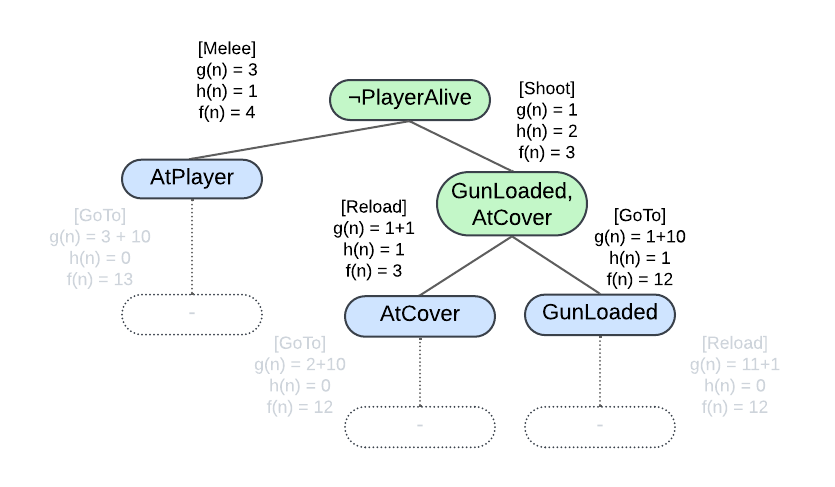
\includegraphics[width=15cm]{GOAP/GOAP_2}
	\captionsetup{justification=justified, format=plain}
  \caption{GOAP A* Suche}
  \label{GOAP A* Suche: Erste Aktionen}
\end{figure}

Für den Knoten \textit{GunLoaded, AtCover} werden nun Aktionen gesucht, die die Zustände des Knoten erfüllen. In dem Beispiel sind es \textit{Reload} und \textit{GoTo}. Auch die Knoten die durch die Aktionen entstehen, werden in die offene Liste hinzugefügt. Erneut wählt A* den Knoten mit den geringsten Kosten $f(n)$ zur Expansion.
\clearpage

\begin{figure}[h]
  \centering
  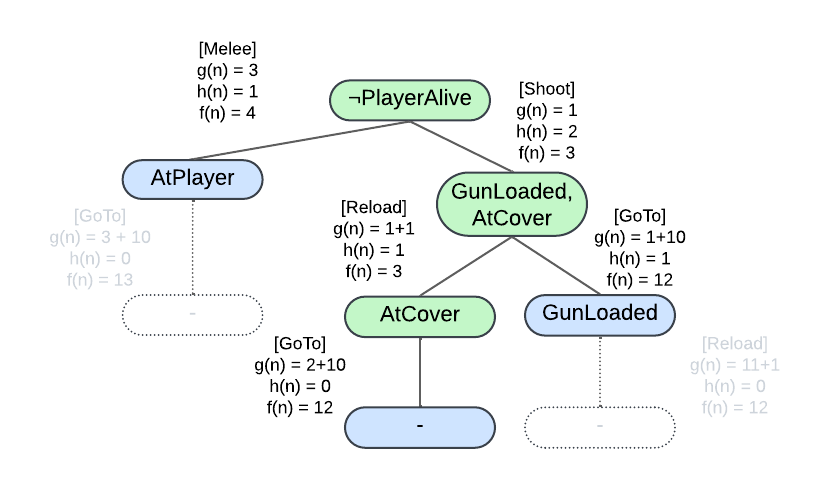
\includegraphics[width=15cm]{GOAP/GOAP_3}
	\captionsetup{justification=justified, format=plain}
  \caption{GOAP A* Suche}
  \label{GOAP A* Suche: Erste Aktionen}
\end{figure}

Der Knoten der durch die Aktion \textit{Reload} entstand, hat dabei die geringsten $f(n)$ Kosten. Der darauf folgende Knoten der durch die Aktion \textit{GoToCover} entsteht hat zwar einen leeren Zustand und wäre somit abgeschlossen, befindet sich aber mit dem \textit{AtPlayer} Knoten, welcher geringere Kosten hat in der offenen Liste.
\clearpage

\begin{figure}[h]
  \centering
  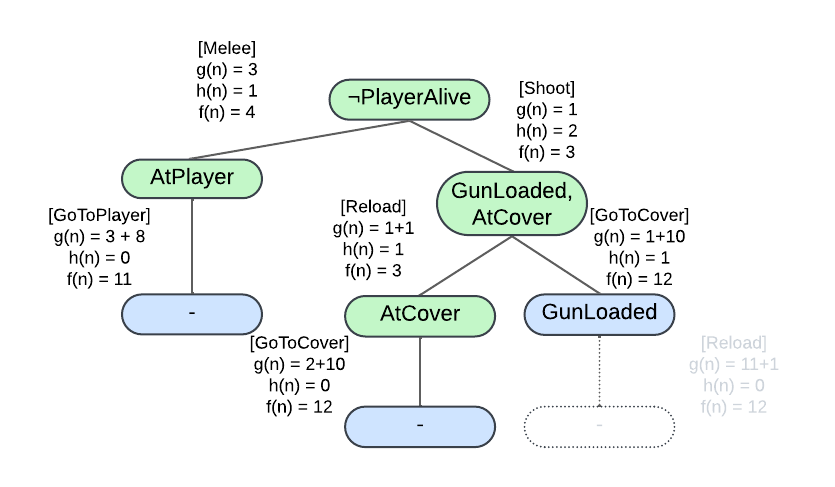
\includegraphics[width=15cm]{GOAP/GOAP_4}
	\captionsetup{justification=justified, format=plain}
  \caption{GOAP A* Suche}
  \label{GOAP A* Suche: Erste Aktionen}
\end{figure}

Aus der offenen Liste wird der nächste Knoten \textit{AtPlayer} gewählt, da dieser die niedrigsten Kosten von allen anderen offenen Knoten hat. Dieser wird durch die Aktion \textit{GoToPlayer} erfüllt und führt zu einem Knoten mit leerem Zustand.

Letztlich wird der günstigste Knoten aus der offenen Liste genommen. Da dieser erfüllt ist, bzw. keine weiteren Zustände besitzt, gibt der Planner nun die Aktionen die zu ihm geführt habe in einer Sequenz zurück. Im Beispiel wäre es die Sequenz: [\textit{Melee, GoToPlayer}].
\clearpage

%\section{Unterschiede STRIPS und GOAP}
%
%Die Hauptunterschiede von STRIPS und GOAP befinden sich dabei bei den eigentlichen Aktionen. Aktionen in GOAP haben Kosten und statt einer Add und Delete List ein Array an Preconditions und Effekten, die den World State verändern.
%
%Aktionen in STRIPS haben im Gegensatz zu GOAP keine Kosten. Anhand der Kosten kann der GOAP Aktionen über andere Aktionen bestimmen. So sollen Aktionen mit geringeren Kosten bevorzugt werden.
%
%STRIPS realisiert Effekte einer Aktion über eine Add und Delete List. Die Delete List löscht Wissen über Zustände. Während die Add List neues Wissen Zustände hinzufügt. In GOAP haben Aktionen Arrays die Preconditions und Effekte speichern. Procedural Preconditions Checks sorgen in GOAP dabei, dass nur Effekte genutzt werden, die erfüllte Preconditions haben. Die Effekte der GOAP Aktionen werden auch nicht direkt umgesetzt. Die Aktionen besitzen eine Funktion, die die Aktion ausführt. Während der Ausführung der Aktion können sich dabei die gewünschten Zustände ändern.